% This is an example of how to create a presentation in PDFLaTeX. 
% Matt Welsh, mdw@cs.berkeley.edu
% See http://www.cs.berkeley.edu/~mdw/proj/texslides for details.

% The basic document style is 'foils' from the FoilTeX package
\documentclass[20pt,landscape]{foils}
% These are my macros for creating slides
\usepackage{mdwslides}

% Basic things that we need are below
\usepackage[english]{babel}
\usepackage{hyperref}
\hypersetup{
  pdfmenubar=true,
  pdftoolbar=true,
  pdfpagemode={None}
}
\usepackage{pause}
\usepackage{graphicx}
\usepackage[utf8]{inputenc}
\inputencoding{utf8}
%%%%%%%%%%%%%%%%%%%%%%%%%%%%%%%%%%%%%%%%%%%%%%%%%%%%%%%%%%%%%%%%%%%%%%%%%%%%

% Set headers
\MyLogo{Ole Aamot}
\rightfooter{\quad\textsf{\thepage}}

\begin{document}
\rm

\slide{}
\LogoOff

\vskip 1.5in
\begin{center}
  {\color{mdwblue}\Large\slingbold Mapping Free Internet Radio for GNOME 3
    \vskip 11ex
    Ole Aamot
    \vskip 1ex
           {\small\trebucit ole@gnome.org}
           \vskip 1ex
                  {\mdwsmall\tt \url{https://people.gnome.org/~ole/GUADEC2017.pdf}
                  }
  }
\end{center}

\slide{Introduction}
\LogoOn
gnome-internet-radio-locator is a Free Software program that allows its users
to easily locate and listen to radio programs on broadcasters on the Internet
such as BBC, KEXP and WMBR, as well as NASA's Third Rock Station and 82 other
Internet Radio stations broadcasting from many universities around the world.

gnome-internet-radio-locator is developed for the GNOME desktop and requires
gst-player from gstreamer (\url{https://gstreamer.freedesktop.org/}) to be installed for audio playback.

gnome-internet-radio-locator is not officially a part of GNU or GNOME,
but using the *.gnome.org infrastructure on\\
\url{http://git.gnome.org/gnome-internet-radio-locator} and\\
\url{https://download.gnome.org/sources/gnome-internet-radio-locator/}

\slide{Why do I write gnome-internet-radio-locator?}

\begin{list1}
\item I am a supporter of
  \begin{list2}
  \item Free Radio
  \item Free Software
  \item Free Speech
  \end{list2}
\item I want to give something back to the Free Software community
\item Internet Radio is a free Internet resource
\item Many Universities run non-profit Internet radio stations
\end{list1}

\slide{History of gnome-internet-radio-locator}

\begin{list1}
\item 2017
  \begin{list2}  
  \item gnome-internet-radio-locator version 0.1.0 was released on April 26th
  \end{list2}
  \begin{list2}
  \item gnome-internet-radio-locator version 0.2.0 was released on June 16th
  \end{list2}    
  \begin{list2}
  \item gnome-internet-radio-locator version 0.3.0 was released on June 20th
  \end{list2}
  \begin{list2}
  \item gnome-internet-radio-locator version 0.4.0 was released on June 27th
  \end{list2}
  \begin{list2}
  \item gnome-internet-radio-locator version 0.5.0 was released on July 17th
  \end{list2}
  \begin{list2}
  \item gnome-internet-radio-locator version 0.6.0 was released on July 19th
  \end{list2}
  \begin{list2}
  \item gnome-internet-radio-locator version 0.7.0 was released on August 4th
  \end{list2}
\end{list1}

\slide{What is the definition of Free Software?}

From FSF's home page (\url{https://www.gnu.org/philosophy/free-sw.html}):

\begin{list1}
\item Free Software is a good idea because you have
  \begin{list2}
    \item The freedom to run the program as you wish, for any purpose (freedom 0).
    \item The freedom to study how the program works, and change it so it does your computing as you wish (freedom 1). Access to the source code is a precondition for this.
    \item The freedom to redistribute copies so you can help your neighbor (freedom 2).
    \item The freedom to distribute copies of your modified versions to others (freedom 3). By doing this you can give the whole community a chance to benefit from your changes. Access to the source code is a precondition for this.
  \end{list2}
\end{list1}

\slide{Existing Music Services}

\begin{list1}
\item Apple Music, Google Music and Spotify
  \begin{list2}
  \item Require non-free client software
  \item DRM (Digital Restrictions Management)
  \item Impose EULAs that restrict more than copyright
  \item Track what the user listens to
  \end{list2}
\end{list1}

One redeeming feature of some of them:

\begin{list2}
\item You can't access them from GNU/Linux at all.  If you're a GNU/Linux user, this protects you from the temptation to use them.
\end{list2}

\slide{Why did I write gnome-internet-radio-locator?}

The last public talk I gave in the UK, was a talk on Music Recording, Production and Distribution with Free Software at UKUUG Linux 2005 at University of Wales, Swansea, in 2005. The talk is available from \url{http://home.nuug.no/~ole/UKUUG2005.pdf}

12 years is a long time, a lot of stuff has happened in these 12 years.

\begin{list1}
\item Free Radio
\item Free Software
\item Free Speech
\end{list1}

\slide{Features in gnome-internet-radio-locator version 0.7.0}

\begin{list1}
\item 86 non-profit and independent radio stations are supported.
\item 10 language translations (see gnome-internet-radio-locator/AUTHORS and gnome-internet-radio-locator/THANKS).
\item Radio station search by physical location, but just city names.
\item Click-to-play map feature for KALX in Berkeley, CA and WAMU in Washington, DC
\item Support for New/Personal Stations (``\$HOME/.gnome-internet-radio-locator/gnome-internet-radio-locator.xml'').
\item Radio playback in all audio codecs supported by gstreamer.
\end{list1}

\slide{Supported Internet Radio Stations}

The following major cities are supported in gnome-internet-radio-locator 0.7.0:

\begin{list1}
\item
  \begin{list2}
    \item Adelaide, Australia
    \item Auckland, New Zealand
    \item Austin, TX
    \item Ayr, Scotland
    \item Bergen, Norway
    \item Berkeley, CA
    \item Bern, Switzerland
    \item Boston, MA
    \item Bristol, United Kingdom
    \item Brno, Czech Republic
    \item Bronx, New York City, NY
    \item Brooklyn, New York City, NY
    \item Bruxelles, Belgium
    \item Budapest, Hungary
    \item Buenos Aires, Argentina
    \item Calgary, Canada
    \item Cambridge, United Kingdom
    \item Cape Town, South Africa
    \item Centralia, DC
    \item Chapel Hill, NC
    \item Chicago, IL
    \item Cleveland, OH
    \item Coimbra, Portugal
    \item Copenhagen, Denmark
    \item Cornwall, United Kingdom
    \item Dublin, Ireland
    \item Gent, Belgium
    \item Guatemala City, Guatemala
    \item Hammond, LA
    \item Honolulu, HI
    \item Houston, TX
    \item Kingston, Canada
    \item Kristiansand, Norway
    \item Leeds, United Kingdom
    \item London, United Kingdom
    \item Long Island, NY
    \item Los Angeles, CA
    \item Lund, Sweden
    \item Manchester, United Kingdom
    \item Memphis, TN
    \item México City, México
    \item Minneapolis, MN
    \item Narvik, Norway
    \item Nashville, TN
    \item Newcastle, Australia
    \item New Orleans, LA
    \item New York City, NY
    \item Nicosia, Cyprus
    \item Nottingham, United Kingdom
    \item Oslo, Norway
    \item Oswego, NY
    \item Ottawa, Canada
    \item Oxford, United Kingdom
    \item Palo Alto, CA
    \item Paris, France
    \item Phoenix, AZ
    \item Pisa, Italy
    \item Pittsburgh, PA
    \item Portland, OR
    \item Reykjavik, Iceland
    \item Rochester, MI
    \item Salford, United Kingdom
    \item San Marcos, TX
    \item Santiago, Chile
    \item São Paulo, Brazil
    \item Seattle, WA
    \item Space
    \item Stockholm, Sweden
    \item St. Pölten, Austria
    \item Sydney, Nova Scotia, Canada
    \item Toronto, Canada
    \item Trondheim, Norway
    \item Tuscaloosa, AL
    \item Washington, DC
    \item Waterloo, Canada
    \item York, United Kingdom
    \item Zürich, Switzerland
  \end{list2}
\end{list1}

See
\begin{tiny}\url{https://people.gnome.org/~ole/gnome-internet-radio-locator/gnome-internet-radio-locator.xml}\end{tiny} for the current list of supported radio stations in gnome-internet-radio-locator.

\slide{Supported Radio Codecs}

The radio stations stream live audio with several different audio codecs supported by the gstreamer program, see \url{https://gstreamer.freedesktop.org/}

The audio codecs in usage among the supported 82 radio stations are:

\begin{list1}
  \item
    \begin{list2}
    \item ``AAC, v4 LC''
    \item ``MPEG 1 Audio, Layer 3 (MP3)''
    \item ``MPEG ADTS, layer III (Joint Stereo)''
    \item ``MPEG-2 AAC (AAC+)''
    \item ``MPEG-2 AAC''
    \item ``MPEG-4 AAC''
    \item ``Ogg Vorbis''
    \end{list2}
\end{list1}

\slide{gnome-internet-radio-locator Data Type Definition (DTD)}

\begin{list1}
\item gnome-internet-radio-locator 0.1.0 DTD
\item Short description of each radio station (<station ...>).
\item Short description of each radio station stream (<stream ...>).
\item gnome-internet-radio-locator 0.1.0 DTD is available from \begin{tiny}\url{https://people.gnome.org/~ole/gnome-internet-radio-locator/gnome-internet-radio-locator-0.1.dtd}\end{tiny}
\item gnome-internet-radio-locator 0.7.0 XML data renders as HTML using XSLT in at least Firefox 54.0 at \begin{tiny}\url{https://people.gnome.org/~ole/gnome-internet-radio-locator/gnome-internet-radio-locator.xml}\end{tiny}
\end{list1}


\slide{Current gnome-internet-radio-locator 0.1.0 DTD}

\begin{tiny}
\begin{verbatim}
<!ATTLIST frequency uri CDATA #REQUIRED >
<!ELEMENT description ( #PCDATA ) >
<!ATTLIST description lang CDATA #REQUIRED >
<!ELEMENT frequency ( #PCDATA ) >
<!ELEMENT email ( #PCDATA ) >
<!ELEMENT location ( lat | lon | href)* >
<!ELEMENT gnome_internet_radio_locator ( station+ ) >
<!ATTLIST gnome_internet_radio_locator version NMTOKEN #REQUIRED >
<!ELEMENT station ( frequency | location | description | stream)* >
<!ATTLIST station band CDATA #REQUIRED >
<!ATTLIST station icon CDATA #REQUIRED >
<!ATTLIST station id NMTOKEN #REQUIRED >
<!ATTLIST station lang CDATA #REQUIRED >
<!ATTLIST station name CDATA #REQUIRED >
<!ATTLIST station rank CDATA #REQUIRED >
<!ATTLIST station type CDATA #REQUIRED >
<!ELEMENT stream EMPTY >
<!ATTLIST stream bitrate NMTOKEN #REQUIRED >
<!ATTLIST stream channels NMTOKEN #IMPLIED >
<!ATTLIST stream codec CDATA #REQUIRED >
<!ATTLIST stream mime CDATA #REQUIRED >
<!ATTLIST stream samplerate NMTOKEN #REQUIRED >
<!ATTLIST stream uri CDATA #REQUIRED >
\end{verbatim}
\end{tiny}

\slide{Example of gnome-internet-radio-locator 0.7.0 XML data}

\begin{tiny}
\begin{verbatim}
<?xml version="1.0" encoding="UTF-8"?>
<?xml-stylesheet type="text/xsl"
  href="https://people.gnome.org/~ole/gnome-internet-radio-locator/gnome-internet-radio-locator.xsl" ?>
<!DOCTYPE gnome-internet-radio-locator SYSTEM "gnome-internet-radio-locator-0.1.dtd">
<gnome_internet_radio_locator version="0.7.0">
  ...
  <station band="88.1FM"
           id="wmbr"
           lang="en"
           name="WMBR"
           rank="1.0"
           type="edu">
    <frequency>88.1 FM in Cambridge, MA</frequency>
    <location>Boston, MA</location>
    <description lang="en">WMBR is the MIT campus radio station.
    We broadcast on 88.1 FM between 20 and 24 hours per day, 365 days a year.
    We transmit at 720 watts, effective radiated power from the top of the
    Eastgate Building in Kendall Square in Cambridge, Massachusetts.
    Our programming includes a wide range of music shows, public affairs
    programs and eclectic audio entertainment.</description>
    <stream mime="audio/mpeg"
            uri="http://wmbr.org/WMBR_live_128.m3u"
            codec="MPEG 1 Audio, Layer 3 (MP3)"
            samplerate="44100 Hz"
            channels="Stereo"
            bitrate="128 kbps" />
    <uri>http://wmbr.org/</uri>
  </station>
  ...
</gnome_internet_radio_locator>
\end{verbatim}
\end{tiny}

\slide{Screenshot}

\begin{center}

  \colorbox{white}{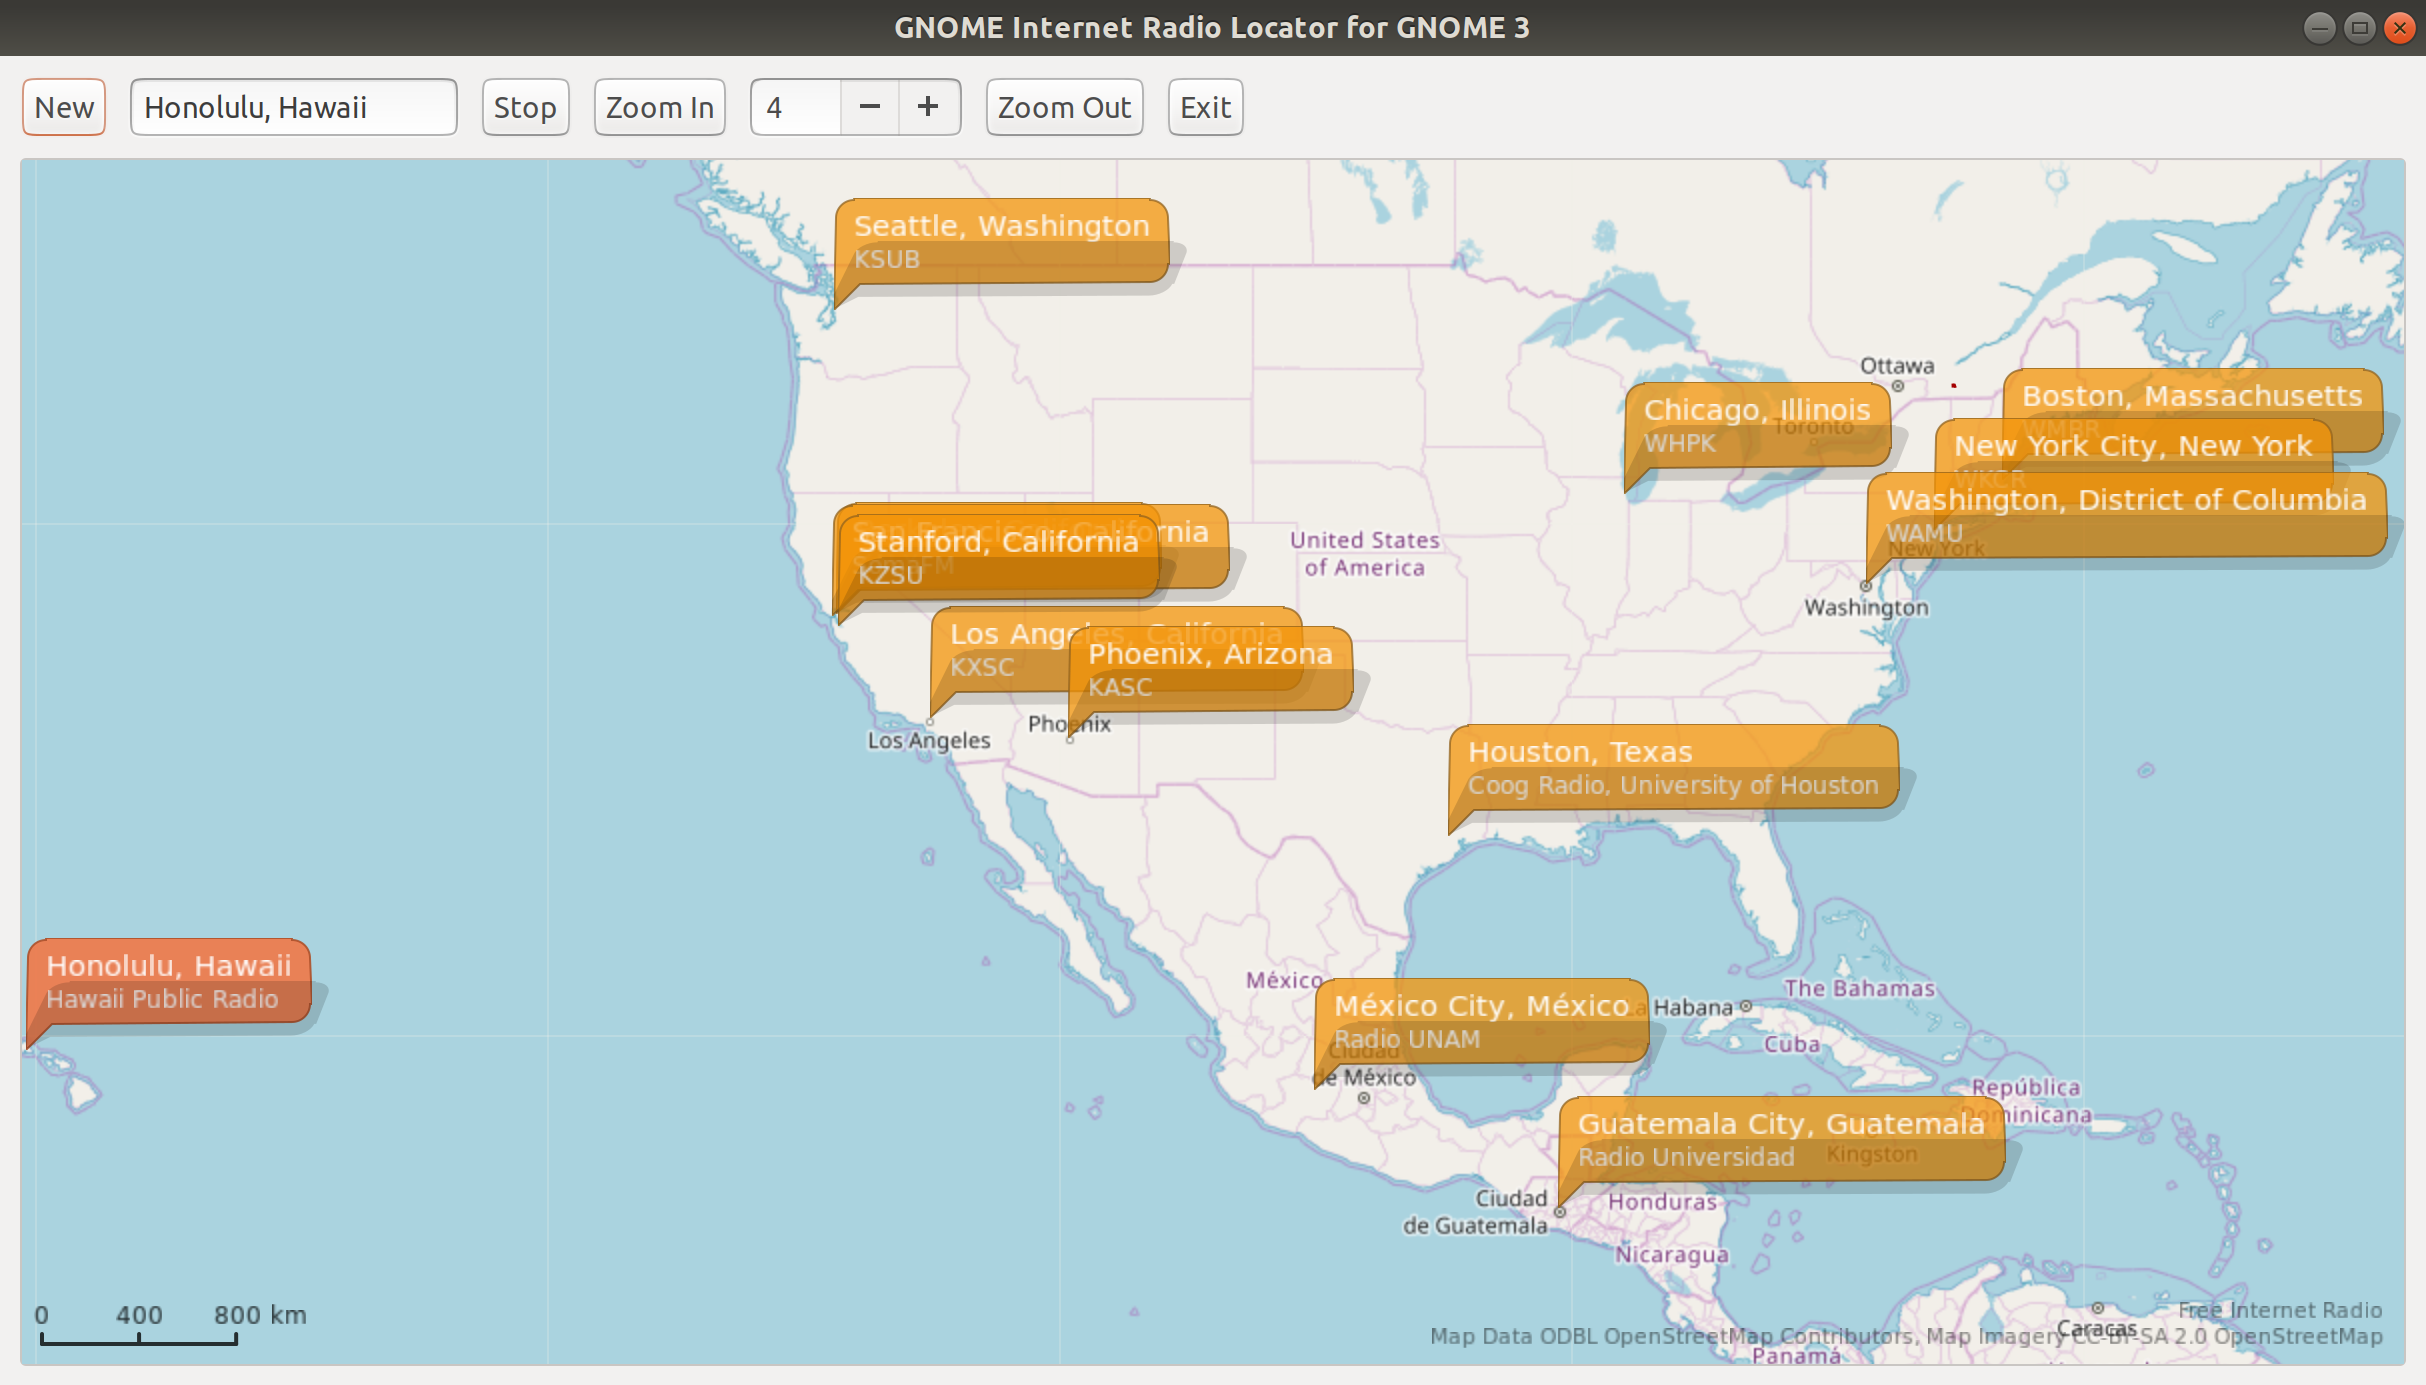
\includegraphics[width=0.6\hsize]{../data/screenshot.png}}

  {\blueem Screenshot of gnome-internet-radio-locator 0.7.0}

\end{center}

\slide{Legal stuff}

\begin{list1}
  \item Internet Radio stations in the U.S. need a broadcast license permit from the F.C.C.
    \begin{list2}
    \item Read gnome-internet-radio-locator/BROADCAST for some details on radio and music licensing
    \item \url{http://en.wikipedia.org/wiki/Broadcast_license}
    \item \url{https://www.dnalounge.com/backstage/webcasting.html}
    \end{list2}
  \item Personal Radio Stations can be set up using Icecast streaming server
    \begin{list2}
    \item Download Icecast from \url{http://www.icecast.org/} and add your station in \$HOME/.gnome-internet-radio-locator/gnome-internet-radio-locator.xml
    \end{list2}
  \item Only Internet radio stations with broadcast permit are included in gnome-internet-radio-locator
\end{list1}

\slide{Internet Radio Fairness Act}

\begin{list1}
\item Many Internet radio stations can't afford to pay royalty fee collection agencies
  \begin{list2}
  \item The American Society of Composers, Authors and Publishers (ASCAP)
  \item Broadcast Music, Inc. (BMI)
    \item Society of European Stage Authors and Composers (SESAC)
  \end{list2}
  \item New bill in support of Internet Radio introduced in U.S. Congress 2002:
  \begin{list2}
  \item \url{https://www.eff.org/Internet-Radio-Fairness-Act-Explanation}
  \item \url{http://en.wikipedia.org/wiki/Internet_Radio_Equality_Act}
  \end{list2}
\item EFF had a 2012 campaign in support of the Internet Radio Fairness Act
  \begin{list2}
  \item \url{https://www.eff.org/Internet-Radio-Fairness-Act-Explanation}
  \end{list2}
\item The IRFA bill may be reintroduced in U.S. Congress in 2017, but who knows?
\end{list1}

\slide{Email from Dr. Richard M. Stallman of FSF}

\begin{list1}
\item
  \begin{tiny}
\begin{verbatim}
    From: Richard Stallman <rms@gnu.org>
    Subject: Re: Internet Radio Fairness Act? (Re: It's your birthday)
    Date: Mon, 23 Mar 2015 22:43:25 -0400
    To: oka@oka.no

    [[[ To any NSA and FBI agents reading my email: please consider    ]]]
    [[[ whether defending the US Constitution against all enemies,     ]]]
    [[[ foreign or domestic, requires you to follow Snowden's example. ]]]

      > Regarding updating the LETTER included in GNOME Internet Radio Locator,
      > I don't know what to write/who to contact to promote Internet Radio
      > Fairness Act again in U.S. politics, except you.

    Ask people to contact their congressional representatives.

    Can you write a message to the public about this?

    -- 
    Dr Richard Stallman
    President, Free Software Foundation
    51 Franklin St
    Boston MA 02110
    USA
    www.fsf.org  www.gnu.org
    Skype: No way! See stallman.org/skype.html.
\end{verbatim}
  \end{tiny}
\end{list1}  

\slide{Questions?}

\begin{list1}
\item gnome-internet-radio-locator 0.7 is available here and now.
  \begin{list2}
  \item \begin{tiny}\url{http://download.gnome.org/sources/gnome-internet-radio-locator/0.7/gnome-internet-radio-locator-0.7.0.tar.xz}\end{tiny}
  \end{list2}
\item Debian testing package
  \begin{list2}
  \item \begin{tiny}\url{https://people.gnome.org/~ole/gnome-internet-radio-locator/debian/gnome-internet-radio-locator_0.7.0-1_i386.deb}\end{tiny}
  \end{list2}
\item Fedora 26 RPM
  \begin{list2}
  \item \begin{tiny}\url{https://people.gnome.org/~ole/gnome-internet-radio-locator/gnome-internet-radio-locator-0.7.0-1.fc26.x86_64.rpm}\end{tiny}
  \end{list2}
\item Ubuntu 17.04 package
  \begin{list2}
  \item \begin{tiny}\url{https://people.gnome.org/~ole/gnome-internet-radio-locator/gnome-internet-radio-locator_0.7.0-1_amd64.deb}\end{tiny}
  \end{list2}
\item Source repository
  \begin{list2}
    \item \url{git://git.gnome.org/gnome-internet-radio-locator}
    \item \url{https://git.gnome.org/browse/gnome-internet-radio-locator}
    \item \url{ssh://$USERNAME@git.gnome.org/git/gnome-internet-radio-locator}
  \end{list2}
\item Mailing List for gnome-internet-radio-locator is pending\\
  \begin{list2}
  \item See Bugzilla \#781841: \begin{tiny}\url{https://bugzilla.gnome.org/show_bug.cgi?id=781841}\begin{verbatim}

I published the 0.2.0 release of gnome-internet-radio-locator in
  
https://download.gnome.org/sources/gnome-internet-radio-locator/
  
I would like the mailing list for the project to be created as
gnome-internet-radio-locator-list@gnome.org to correspond with
the correct name of the project: gnome-internet-radio-locator

I have already referred to
http://mail.gnome.org/mailman/listinfo/gnome-internet-radio-locator-list
in gnome-internet-radio-locator.doap

<mailing-list rdf:resource=''http://mail.gnome.org/mailman/listinfo/gnome-internet-radio-locator-list'' />

I maintain the source tree in GNOME git on https://git.gnome.org//browse/gnome-internet-radio-locator/

Thanks in advance.

Happy hacking,
Ole
\end{verbatim}
\end{tiny}
  \item \begin{tiny}\url{http://mail.gnome.org/mailman/listinfo/gnome-internet-radio-locator-list/}\end{tiny}    
  \end{list2}  
\end{list1}

\slide{\LaTeX{} source code for this presentation}

\url{https://git.gnome.org/browse/gnome-internet-radio-locator/plain/talk/GUADEC2017.tex}

\slide{GNOME Wiki page}

\url{https://wiki.gnome.org/Apps/GNOMEInternetRadioLocator}

\end{document}
